\documentclass[tikz,border=0pt]{standalone}
\usepackage[T1]{fontenc}
\usepackage{tgheros}
\usepackage{newtxmath}
\usetikzlibrary{arrows.meta}
\renewcommand{\familydefault}{\sfdefault}

\definecolor{ink}{HTML}{172C3D}
\definecolor{muted}{HTML}{4D626F}
\definecolor{news}{HTML}{147D75}
\definecolor{newsPanel}{HTML}{EAF6F3}
\definecolor{newsBorder}{HTML}{A6CBC4}
\definecolor{risk}{HTML}{9B5C21}
\definecolor{riskPanel}{HTML}{FFF4E7}
\definecolor{riskBorder}{HTML}{DBC1A2}
\definecolor{outputPanel}{HTML}{EDF3F8}
\definecolor{outputBorder}{HTML}{A5B8C9}
\definecolor{cash}{HTML}{D4DEE7}

\begin{document}
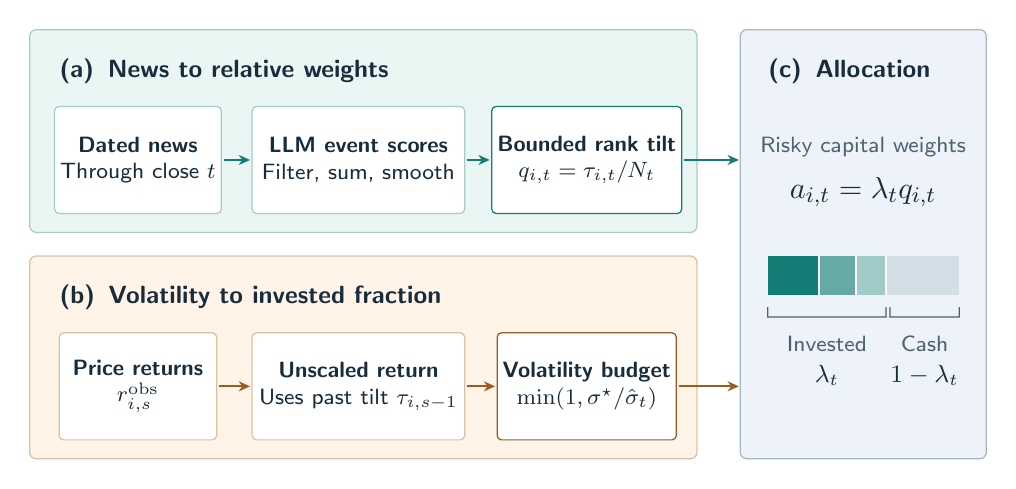
\begin{tikzpicture}[
  x=1mm,y=1mm,text=ink,
  heading/.style={anchor=west,inner sep=0pt,font=\sffamily\bfseries\fontsize{9}{10}\selectfont},
  stage/.style={fill=white,draw,line width=.45pt,rounded corners=1.6pt,
    minimum height=13.6mm,align=center,inner sep=2pt,
    font=\sffamily\fontsize{8.1}{10}\selectfont},
  detail/.style={font=\sffamily\fontsize{7.6}{9}\selectfont,text=muted,inner sep=0pt},
  connector/.style={-{Stealth[length=4.1pt,width=3.6pt]},line width=.8pt,
    shorten <=.65pt,shorten >=.5pt},
  bracket/.style={draw=muted,line width=.45pt}
]
\path[use as bounding box] (0,0) rectangle (122,55);

% The two rules feed separate inputs into one capital allocation.
\draw[fill=newsPanel,draw=newsBorder,line width=.45pt,rounded corners=2.4pt]
  (.25,29) rectangle (85,54.75);
\draw[fill=riskPanel,draw=riskBorder,line width=.45pt,rounded corners=2.4pt]
  (.25,.25) rectangle (85,26);
\draw[fill=outputPanel,draw=outputBorder,line width=.45pt,rounded corners=2.4pt]
  (90.5,.25) rectangle (121.75,54.75);

\node[heading] at (4,49.5) {(a)\enspace News to relative weights};
\node[heading] at (4,20.75) {(b)\enspace Volatility to invested fraction};
\node[heading] at (94,49.5) {(c)\enspace Allocation};

\node[stage,draw=newsBorder,minimum width=20mm] (newsInput) at (14,38.2)
  {\textbf{Dated news}\\[-.4pt] Through close $t$};
\node[stage,draw=newsBorder,minimum width=27mm] (score) at (42,38.2)
  {\textbf{LLM event scores}\\[-.4pt] Filter, sum, smooth};
\node[stage,draw=news,minimum width=22mm] (rank) at (71,38.2)
  {\textbf{Bounded rank tilt}\\[-.4pt] $q_{i,t}=\tau_{i,t}/N_t$};

\node[stage,draw=riskBorder,minimum width=20mm] (price) at (14,9.45)
  {\textbf{Price returns}\\[-.4pt] $r^{\mathrm{obs}}_{i,s}$};
\node[stage,draw=riskBorder,minimum width=27mm] (history) at (42,9.45)
  {\textbf{Unscaled return}\\[-.4pt] Uses past tilt $\tau_{i,s-1}$};
\node[stage,draw=risk,minimum width=22mm] (budget) at (71,9.45)
  {\textbf{Volatility budget}\\[-.4pt] $\min(1,\sigma^\star/\hat\sigma_t)$};

\draw[connector,news] (newsInput.east) -- (score.west);
\draw[connector,news] (score.east) -- (rank.west);
\draw[connector,news] (rank.east) -- (90.5,38.2);
\draw[connector,risk] (price.east) -- (history.west);
\draw[connector,risk] (history.east) -- (budget.west);
\draw[connector,risk] (budget.east) -- (90.5,9.45);

\node[detail] at (106.1,39.8) {Risky capital weights};
\node[font=\fontsize{11}{12}\selectfont,inner sep=0pt] at (106.1,34.1)
  {$a_{i,t}=\lambda_t q_{i,t}$};

% Illustrative capital split, with the invested and cash amounts labelled.
\fill[news] (94,21) rectangle (100.5,26);
\fill[news!65!white] (100.5,21) rectangle (105.2,26);
\fill[news!40!white] (105.2,21) rectangle (109,26);
\fill[cash] (109,21) rectangle (118.3,26);
\draw[white,line width=.45pt] (100.5,21) -- (100.5,26)
  (105.2,21) -- (105.2,26) (109,21) -- (109,26);
\draw[bracket] (94,19.5) -- ++(0,-1.25) -- (109,18.25) -- (109,19.5);
\draw[bracket] (109.5,19.5) -- ++(0,-1.25) -- (118.3,18.25) -- (118.3,19.5);
\node[detail] at (101.5,14.9) {Invested};
\node[detail] at (113.9,14.9) {Cash};
\node[font=\fontsize{8.6}{10}\selectfont,inner sep=0pt] at (101.5,10.8)
  {$\lambda_t$};
\node[font=\fontsize{8.6}{10}\selectfont,inner sep=0pt] at (113.9,10.8)
  {$1-\lambda_t$};
\end{tikzpicture}
\end{document}
